%auto-ignore
%      this ensures the arxiv doesn't try to start TeXing here.
%!TEX root = super_lattice_models_draft.tex
%      prev line helps TeXShop do the right thing

%%%%%%%%%%%%%%%%
\section{Kitaev chain} \label{kitaev_wire}
%%%%%%%%%%%%%%%%
\dave{Should remark somwhere in this section (or in the apprpriate places) that we haven't put any effort into normalizing our wavefunctions in this section.}
\dave{After reading through once again it looks like none of our wavefunctions are normalized.}

In this section, we show how the graphical formalism developed in previous sections
can be used to capture the salient features of the `Kitaev wire', 
Kitaev's toy model of a one-dimensional spinless $p$-wave superconductor \cite{kitaev2001}. 
This highlights the connection between Majorana zero modes and Ising anyons and serves 
as a nice application of the graphical calculus of the $C_2$ theory.
Most of what we say applies beyond the $C_2$ theory and can be carried out for any theory containing at least one $q$-type object.
%  although the procedure we work 
%out can be carried out for any theory containing at least one $q$-type object.
%, and provides 
%a simple (alas, perhaps too simple) illustration of the shadow world approach detailed in the previous section 
%(with appropriate modifications for the reduced dimensionality of the problem). 
The Hamiltonian we write down is the same as the one constructed in \ref{Super_pivotal_Hamiltonian}, with a cell decomposition of a disk (annulus) with fixed boundary conditions\dave{Maybe draw picture?}.
Correspondingly, the associated wavefunctions we construct
%and the associated wavefunctions we construct are 
are the same as those found in e.g. \cite{fidkowski2011}, but presented in a more graphical formalism 
and serve as a simple example of the techniques discussed in Section \ref{state_sums}.
%and 
%discussed within the framework of the tools developed in this paper. 

Recall that the $C_2$ theory has two simple objects $\unit,\beta$,
with $\beta\tp \beta\cong \cc^{1|1}\unit$,
and $\End(\beta) \cong \cliff_1$.
%We will see that the $\beta$ object plays the role of a Majorana fermion in the Kitaev wire, with a strand 
%of $\beta$ string being described by the physics of the Kitaev wire. 
We will focus on the $\beta$ object in the $C_2$ 
theory for concreteness, but the analysis can be applied q-type objects $q$ in any theory.
% that satisfy $q\tp q \cong \cc^{1|1} \unit \oplus \dots$.
%\dave{ Probably don't need the last bit, but could say: $q\tp q^* \cong \cc^{1|1} \unit \oplus \dots$}

In what follows, 
we will show that a single strand of $\beta$ string is a diagrammatic description for the zero correlation length limit of the Kitaev chain. 
%\dave{I think Kapustin/Thorngren have a paper that mention something along these lines should probably cite them.} \ethan{yes, they did. I had the reference somewhere... added it back}.
This means that the string-net Hamiltonian in Section \ref{Super_pivotal_Hamiltonian} 
based on the $C_2$ theory describes a phase of fluctuating Kitaev wires, 
an idea previously investigated in \cite{tarantino2016,ware2016,kapustin2017}.

The basic strategy is to cut a single $\beta$ strand into pieces and analyze how to glue those pieces back together to recover the uncut strand.
Physically, we will implement the gluing by requiring the vectors to be in the ground space of a particular Hamiltonian -- similar to what we did in Section \ref{Super_pivotal_Hamiltonian}. 
%the Hamiltonian which glues those pieces back together.
% and examine what must be done to glue the 
%pieces back together.
%Versions of these sentences have been constructed elsewhere
%Algebraically, this contraint is just $\tp_{\End(\beta)}$, 
%physically we can impliment this constraint by taking a free tensor product and project into the ground space of a Hamiltonian implimenting that constraint. 
%The Hamiltonian turns out to be a limiting case of the Kitaev wire, the zero correlation length limit.
We first note that the vector space associated to a single interval $I$ with boundary conditions labeled by $\beta$ can be written graphically as 
\be\label{VIbetabeta}
 A(I;\beta,\beta) = \cc \left[ \halfchain\;, \; \halfchaindot \right] \cong \cc^{1|1}.\ee
 
 Now we can consider splitting the interval $I$ into two smaller intervals $I_1,I_2$, such that $I_1\cup I_2 = I$.
 We then can reconstruct the vector space $A(I;\beta,\beta)$ from the vector 
 spaces $A(I_1;\beta,\beta),A(I_2;\beta,\beta)$ by gluing the two intervals $I_1,I_2$ together. 
Algebraically, this gluing is implemented by the tensor product. However, 
we must be sure to make the proper choice 
of tensor product to ensure that we don't produce any extra degrees of freedom during the gluing. 
The standard tensor product $\tp_\cc$ doesn't work, since then $A(I_1;\beta,\beta) \tp_\cc A(I_2;\beta,\beta) \cong \cliff_2 \not\cong A(I;\beta,\beta)$. 

The correct tensor product to use is the relative tensor product $\tp_{\End(\beta)}$ (a.k.a $\tp_{\cliff_1}$) discussed in Section \ref{modified_tensor_product}. 
With this tensor product, we (rather trivially) have 
%We thus can write 
\be A(I;\beta,\beta) \cong A(I_1;\beta,\beta) \tp_{\End(\beta)} A(I_2;\beta,\beta),\ee
which tells us how to split apart the $I$ interval correctly. 

Graphically, the relative tensor product $\tp_{\End(\beta)}$  is needed to mod out by local relations involving the sliding of fermions along $\beta$ lines, 
as was discussed Section \ref{modified_tensor_product}. 
%where the relative tensor product $\tp_{\End(\beta)}$ (a.k.a $\tp_{\cliff_1}$) is needed to mod out by local relations involving the sliding of fermions along $\beta$ lines, 
%as was discussed at length in Section \ref{modified_tensor_product}. 
Utilizing $\tp_{\End(\beta)}$ is equivalent to performing the regular tensor product $\tp_\cc$ and modding out by the equivalence relations
\begin{align}
\label{graphical_equiv_reln} 
\halfchain \tp_\cc \halfchaindot \; &=\; \halfchaindot \tp_\cc \halfchain\; ,\\%\quad \quad \text{,}\\
\nonumber
\halfchaindot \tp_{\cc} \halfchaindot \;  &= -A^4\; \halfchain \tp_{\cc}  \halfchain.
\end{align}
where we have assumed a Koszul ordering for the fermions which increases from left to right (see Table \ref{C2_data_table} for the origin of the phase $A^4$).
%\be
% \horizbeta \tp_\cc \horizbetadot  \sim  \horizbeta \tp_\cc \horizbeta\;.
%\ee

As we did with the string-net Hamiltonian in Section \ref{Super_pivotal_Hamiltonian}, 
we can implement these equivalence relations energetically, via an appropriately defined Hamiltonian.

%\dave{Changed $N$ to little $n$ since B(N) spin structures}
%\ethan{cool}
Consider an interval $I$ of $\beta$ string cut into $n$ segments: $I = I_1\cup I_2\cup\dots\cup I_n$.
Each segment $I_i$ will end up mapping to a single physical site in the Kitaev chain. 
The local Hilbert space at each $I_i$ segment is generated by two basis vectors $v_e,v_o$, 
which for convenience we draw as
\begin{align} \label{vevodefn}
v_e \; = \;\LocalHilba\,,\qquad v_o \; = \; \LocalHilbb\;.
\end{align}
The upward-curved ends on each $\beta$ segment are drawn purely for aesthetic purposes, and exist solely to make drawing the Kitaev chain slightly easier. 
The local Hilbert space is then
%\dave{I don't think we use the notation $\langle v_e,v_o\rangle $ anywhere else in the paper.}
\begin{align}
A(I_i; \beta, \beta) = \cc \left[ \LocalHilba, \LocalHilbb \right] \cong \cc^{1|1}.
\end{align}


The total Hilbert space of the chain is given by tensoring each local Hilbert space together:
\begin{align} 
\label{HilbInterval}
\mch_I  = A(I_1; \beta, \beta)  \tp_\cc A(I_2; \beta, \beta)  \tp_\cc \cdots \tp_\cc A(I_n; \beta, \beta).  
\end{align} 
States in this Hilbert space are expressed graphically as
%\dave{Fix LHS.}
\begin{align} \label{example_hilb_vectors}
\quarterpiperprime \tp  \LocalHilba \tp  \LocalHilba \tp  &\cdots \tp  \LocalHilba \tp  \quarterpipelprime, \\
\quarterpiperdotprime \tp  \LocalHilbb \tp  \LocalHilba \tp  &\cdots \tp  \LocalHilba \tp  \quarterpipelprime, \\
\quarterpiperdotprime \tp  \LocalHilba \tp  \LocalHilbb \tp  &\cdots \tp  \LocalHilba \tp  \quarterpipelprime, \\
&\;\; \vdots
\end{align}
and so on. 
%\dave{over-complete and too large sound kind of weird, might want to change at some point.}
Instead of using the relative tensor product $\tp_{\End(\beta)}$ to mod out by the equivalence relations \eqref{graphical_equiv_reln} we use $\tp_\cc$ (abbreviated as $\tp$ above) and define a Hamiltonian so that the ground space is isomorphic to $A(I, \beta, \beta)$. 
%we define a Hamiltonian whose  agrees with the TQFT Hilbert space  
%Since we used $\tp_\cc$ when writing the above states, these states are over-complete: we have not yet modded out by the equivalence relations \eqref{graphical_equiv_reln}.
%However, this Hilbert space is too large, since we have not yet modded out by the equivalence relations \eqref{graphical_equiv_reln}. 
%Instead of using the relative tensor product to do this, we can make use of the projectors
The Hamiltonian is just the one-dimensional version of the edge term in \eqref{ham} and can be written as:
\begin{align} \label{kitaev_chain_ham_sitei}
H_i =  \frac{1}{2} \left( \Id \;\; + \;\; \TwoLinedotdot \right),
\end{align}
which have a non-trivial action only on the adjacent Hilbert spaces associated to the intervals $I_i$ and $I_{i+1}$.
%where the left lines are applied to right end of the $i$th strand and the right lines are applied to the left end of the $(i+1)$-th strand
\footnote{Note that there are no terms that act on both the right and left ends of a single strand/interval; such a term would perturb us away from the zero correlation length limit.
%---the absence of such terms is because we are working in topological phase of the Kitaev chain in the completely staggered limit. 
In the language of the Kitaev chain, this corresponds to tuning the chemical potential to zero and the 
magnitude of the superconducting gap to the hopping amplitude.}.
%\ethan{I am in favor of writing the Hamiltonian like this, with the understanding that when we draw pictures and stuff, we are modding out by fermion slides and that the spin framing is fixed so that we have the usual $C_2$ diagrammatic manipulations. We can talk about $\alpha(e)$ stuff and edge terms to implement endos etc, but I think we probably shouldn't}

The image of this projector on a pair of adjacent string endpoints is  
%\ethan{may want to fix dotted quarterpipes in this equation as well}
%\dave{I think it's fine, but could change it if you want.}
%\ethan{nah, guess it's fine}
\begin{align} 
\quarterpiper \tp_\cc \quarterpipel + \quarterpiperdot \tp_\cc \quarterpipeldot = \halfchain \tp_{\End(\beta)} \halfchain,
\end{align}
so that using $\tp_\cc$ and projecting with $H$ is equivalent to using $\tp_{\End(\beta)}$. %(in Section \ref{Super_pivotal_Hamiltonian}, the $(1-D_e)$ term played the role of $H$).
%\dave{commented on this above}. 
Thus, $H_i$ is responsible for gluing together ends of $\beta$ strands. 
In terms of electronic operators, $H_i$ implements hopping and pairing between electrons in nearest neighbor sites $i$ and $i+1$.

We form our Hamiltonian from a sum of projectors, $H_i$, acting between each pair of strands:
\begin{align}
\label{KWHam}
H = t \sum_{i = 1}^{n-1} (1- H_i).
\end{align}
This Hamiltonian describes the zero correlation length limit of the Kitaev chain, albeit in a slightly unconventional language.
To understand this, we proceed to investigate the ground state wave functions.
%Note that if we replace $C_2$ by an arbitrary super pivotal fusion category $\spc$, 
%and $\beta$ by another q-type object in $\spc$, the Hamiltonian would look the same as above. 
%It would also still have a similar interpretation as a Kitaev chain, where the local Hamiltonian terms induce pairing and hopping on the fermions, but the


%Each $H_i$ contains two terms: the first is the identity operator, while the second is nontrivial and is identified with $i \gamma_1 \gamma_2$, 
%a Majorana bilinear which acts as the fermion parity operator $(-1)^F$ on the on-site Hilbert space.
%It is useful to define a fermion parity operator $(-1)^F$ for each interval.
We note that the nontrivial term in the Hamiltonian is proportional to the fermion parity measured between adjacent physical sites. 
Indeed, acting with that term on the vectors $v_e,v_o$ defined in \eqref{vevodefn}, we find
%To see this, we can simply check the action of the second term on the basis vectors of the single (physical) site Hilbert space. 
%Graphically, the  
%second term acts by stacking diagrams onto input states, and so it acts
%on single-site basis states as
%\begin{align}
%\TwoLinedotdot\; \circ \; \CupSigma \; =\;  \CupSigma \quad \text{and} \quad \TwoLinedotdot\; \circ\; %\CupSigmadot \; =\;   - \; \CupSigmadot.
%\end{align}
\begin{align}
\TwoLinedotdot\; \circ \; v_e =\; v_e \quad \text{and} \quad \TwoLinedotdot\; \circ\; v_o \; =\;   - \; v_o.
\end{align}
which is precisely the action of $(-1)^F$ (which can be identified with $i\gamma_1\gamma_2$ in the conventional Clifford algebra language).
%This is precisely the action of the Majorana bilinear $i\gamma_1\gamma_2 = (-1)^F$.

%\ethan{commented out part about Hermitian-ness since it's obvious. What the hell was I thinking with this paragraph? We'll never know.}
%\dave{Note to self: still need to check this.}
%\ethan{note to self: this is nonsense!}
%In order to show that the Hamiltonian is Hermitian, we need to define a graphical way of implementing 
%Hermitian conjugation. We define the Hermitian conjugate of a diagram to be its reflection about 
%the horizontal axis, with the action of reflection determined by the properties of the complex line 
%bundle constructed in Appendix \ref{fermion_line_bundle} (for more details on the reflection structure, see Section \ref{reflection_ss}). One then verifies that $H^\dagger H = -\lambda^2 \unit$, where the 
%minus sign is a Koszul sign, $\lambda$ is the phase picked up when removing a pair of fermions 
%as in \eqref{removing_fermions}. 
%As usual, the notation $H^\dagger H$ graphically corresponds to stacking $H^\dagger$ on top of $H$.
%Since $\lambda^2 = -1$ as we prove in Appendix \ref{fib_appendix}, we verify that $H^\dagger H = \unit$.  

It is straightforward to find the ground states of \ref{KWHam}.
Noting that the non-trivial term in the Hamiltonian is just measuring the parity shared between adjacent ``physical" sites, 
we can do a change of basis using an F-move so that the Hamiltonian is diagonal and annihilates the ground state.
%find the ground states of this Hamiltonian: there are two zero-energy ground states, differing by their fermion parity:
%One finds two ground states
In this basis the (un-normalized) ground state wavefunctions take the form
%\begin{align} \label{kitaev_wire_ground_states}
%\Psi_e = \;\StaggaredGSEven \; \cdots \; \StaggaredGSEvenR\;, 
%\qquad \text{and} \qquad 
%\Psi_o =\; \StaggaredGSOdd \; \cdots  \; \StaggaredGSEvenR\;.
%\end{align}
\begin{align} \label{kitaev_wire_ground_states}
\Psi_e = \;\StaggaredGSEvenprime \; \cdots \; \StaggaredGSEvenRprime\;, 
\qquad \text{and} \qquad 
\Psi_o =\; \StaggaredGSOddprime \; \cdots  \; \StaggaredGSEvenRprime\;.
\end{align}
In this basis the Hamiltonian acts as $(1-(-1)^F)$ on each pair of vertical strands, which is clearly zero.

%\dave{Note to self: re-visit this paragraph. 
%Probably want to say something like total fermion number isn't conserved, rather than local. \ethan{I think we want to say the fermion is delocalized, fermion number is still conserved mod 2}
%But need to find a nice way to connect that with shuffling fermions around.}
%\dave{I guess de-localized isn't so-good either since that's the case for usual non-topological band insulators as well.
%We could also just remove the remark -- or make the following comment more accurate: `A nice feature of our diagrammatic notation is that it demonstrates single electron tunneling through the wire at zero energy cost, as one expects for a pair of Majorana zero modes de-localized across a Kitaev chain.'
%}

%Indeed we see that, for example the odd parity state has an additional fermion relative to the even parity state, however it's precise position is not a good quantum number as it can freely shuffel from side to side.
%A nice feature of this diagrammatic notation is that the ``delocalization" of the fermion number in the topological phase of the 
%Kitaev wire is made manifest.
%For example, the fermion in the odd-parity state $\Psi_o$ is not localized: it is free to slide along the bottom $\beta$ line
%from one end of the chain to the other (with the sliding being implemented through the odd elements in $\End(\beta)$, or in the context of \eqref{graphical_equiv_reln} by the use of the modified tensor product $\tp_{\cliff_1}$).
%\dave{didn't follow the parenthetical remark so I removed it.
%Feel free to re-instate -- though it may not be necessary for the discussion.}

%At first glance ... in terms of Hilbert spaces, since each physical site carries a Hilbert space of $\cc^{1|1}$, for a chain with $n$ physical sites we have the naive Hilbert space $\mch \cong \cliff_1^{\otimes n}$, which is far bigger than the total ground state space $\cc^{1|1}$ generated by the vectors $\Psi_e$ and $\Psi_o$. 
%... we are actually using the tensor product $\tp_{\cliff_1}$, so that in fact the degrees of freedom are $\cliff_1 \tp_{\cliff_1}  \dots \tp_{\cliff_1} \cliff_1 \cong \cliff_1$. 

To better understand the wavefunctions $\Psi_e,\Psi_o$, we can apply a series of F-moves to change to the physical ``on-site" basis. \footnote{Recall the physical Hilbert space is associated to $A(I_i,\beta, \beta)$, 
whereas the wavefunctions $\Psi_e,\Psi_o$ are expressed in a basis that's ``shared" between adjacent sites.}
%by applying an $F$-move (see \eqref{cupcap_fmove}) to 
%we can perform a change of basis by applying $F$-moves to 
%each cup-cap pair.% with the $F$-move \eqref{cupcap_fmove}. 
In a Kitaev chain with $n$ physical sites (i.e., $n$ intervals), 
we recover the well known result
\dave{double check normalization.}
\dave{I think this wavefunction is just as un-normalized as the one above.}
\ethan{yes, since we just $F$-moved it}
%\be \Psi_e = \frac{1}{d^{n-1}} \bigotimes_{i=1}^n (-A^4)^{n_f/2} \sum_{\{v_i\}}  v_i,\ee
%\be \Psi_e = \frac{1}{d^{n-1}} \bigotimes_{i=1}^n (A^4)^{n_f/2} \sum_{v_i = v_e,v_o}  v_i,\ee
%\dave{Maybe we should write it as:}
%\ethan{this one's correct with the new convention}
%\dave{Great. }
\begin{align}
\Psi_e = \frac{1}{d^{n-1}} \sum_{\substack{ \{ v_i\} \\  n_f = \text{even} }} (A^4)^{n_f/2} \; v_1 \tp v_2 \tp \cdots \tp v_n
\end{align}
where the sum is over all configurations of $v_i =v_o,v_e$ such that only an even number $n_f$ of odd vectors $v_o$ appear 
in the tensor product, and where $v_e,v_o$ are defined as in \eqref{vevodefn}.
For the odd wavefunction $\Psi_o$, we find 
%\ethan{this one is also correct in the new convention!}
%\dave{Great. }
%\be \Psi_e = \frac{1}{d^{n-1}} \bigotimes_{i=1}^n(-A^4)^{(n_f+1)/2} \sum_{\{v_i\}}  v_i,\ee
%\be \Psi_e = \frac{1}{d^{n-1}} \bigotimes_{i=1}^n(A^4)^{(n_f-1)/2} \sum_{v_i = v_e,v_0}  v_i,\ee
\dave{Same with this one.}
\begin{align}
\Psi_o = \frac{1}{d^{n-1}}\sum_{\substack{ \{ v_i\} \\  n_f = \text{odd} }}  (A^4)^{(n_f-1)/2}\; v_1 \tp v_2 \tp \cdots \tp v_n
\end{align}
where the sum is now restricted so that only an odd number $n_f$ of odd vectors $v_o$ vectors in the tensor product.
From the expressions for $\Psi_e,\Psi_o$ in this basis, we see that they are given by configurations 
that are coherent sums over all fermion parity even and fermion parity odd states, respectively.  
%The simplicity of these wavefunctions is a result of only considering the $C_2$ theory.

%\ethan{talk about KW duality here?}
%\dave{Naw, too much writing.}
%\ethan{yay :--)}

%\dave{added some text here, feel free to edit. I'll need to take another pass at it to polish it up.}
%\ethan{made some stylistic edits}
Note that the fermion dot appearing in $\Psi_o$ of \eqref{kitaev_wire_ground_states} has zero energy (since the Hamiltonian does not act on either the beginning of the first strand in the chain or the end of the last strand), while this is not true for fermion dots 
appearing on the interior cups. 
%\dave{interior intermediate sounds awkward.}
%\dave{Does it actually imply the existence of two zero modes (e.g., symmetry)? I'm going to re-phrase it as a conseqence of two zero modes.}
%Physically, this implies the presence of two Majorana zero modes at the ends of the chain. 
Physically, this is due to the presence of a pair of Majorana zero modes localized at the ends of the chain. 
One can explicitly construct the zero mode operators by considering the odd operators acting on either end of the chain; 
they commute with the Hamiltonian, anti-commute with one another, anti-commute with $(-1)^{F_\text{tot}}$ (the total fermion parity), and up to a pre-factor each square to the identity.
These are exactly the properties of a Majorana zero mode. 
\dave{Still can't think of a nice way to say this.}
%One of the hallmarks of a Kitaev chain is that it can seamlessly `teleport' electrons through a gapped medium\cite{Fu?}.

\ethan{dave probably needs to read again to massage it into something he likes. I added some stuff and changed some things around}
One nice feature of our diagrammatic notation is that it makes the fact that a fermion 
can be delocalized between the two ends of the wire completely manifest. 
%the local fermion number is not a good quantum number completely manifest.
%\dave{Want to say that fermion parity of the ground state is de-localized across the zero modes appearing at the termination of the wire. (fermion parity is usually no local.)}
%One feature of the Kitaev chain that the diagrammatic notation nicely captures is that the local fermion number is not a good quantum number. 
Indeed, the fermion dot in the odd-parity state $\Psi_o$ is not localized: it is free to slide along the bottom $\beta$ line
from one end of the chain to the other, %, with any given position representing the same quantum state.
with the sates $\Psi_e,\Psi_o$ being mapped into one another by adding a single fermion to either the left or the right side of the chain. 
%, and in this case a Majorana zero mode.
%\dave{Maybe move what ever we want to say about fermion parity delocalized across the zero modes to here, rather than above.}
%\ethan{sure}

By considering the same spin chain but using the regular Ising fusion category $A_3$ (rather than the condensed $A_3/\psi$ theory), one finds exactly the transverse field Ising model. 
Fermion condensation provides a map between these two models in the same way the Jordan-Wigner transformation does.
%\dave{could add: `; also noted by \cite{turzillo2016,kapustin2017}', not sure if we need to cite people for this. }.
% from this spin model to the Majorana chain in just the way the Jordan-Wigner transformation takes the transverse field Ising model to the Kitaev chain. 
Of course, we have only discussed the zero correlation length limit, but on-site terms can be added as well, and the analysis caries through, except the zero modes are exponentially localized to the boundary (for a small perturbation).
% and one finds similar results, with the zero modes de-localized, etc.  
In the zero correlation length limit, excited states are easily constructed by putting dots on the intermediate cups. 

%\dave{Changed things a bit here, not totally sold on it, but it may speak more to people who are used to thinking about boundary conditions rather than spin structures.}
%\dave{Also need to double check this.}
%\ethan{made some stylistic edits}
We now turn our attention to the Kitaev chain defined on a circle. 
The bulk of the Hamiltonian is constructed from a sum of projectors defined in \eqref{kitaev_chain_ham_sitei}. %, and the %wavefunctions can be found in a similar manner.
%ground-state wavefunctions 
%have a similar form to those in \eqref{kitaev_wire_ground_states}, except the bottom $\beta$ string 
%forms a closed loop below the series of $\beta$ cups. 
To ``glue" the end points of the interval into a circle, we need to add an additional term across the boundary.
There are two ways to do the gluing, differing from one another by a $2\pi$ rotation of the spin framing
(i.e. a spin flip). 
These choices correspond to the two spin structures on the circle: $S^1_B$ and $S^1_N$, corresponding to anti-periodic and periodic fermionic boundary conditions, respectively.
To define periodic boundary conditions we define $H_{n+1}$, the Hamiltonian term which glues the 
two endpoints of the interval together, by
%\dave{Maybe add a bunch of vertical strands in the middle.}
\begin{align}
H_{n+1}^N = \frac{1}{2}
\left(   \; \HambdR  \cdots \HambdL \quad  +  \quad 
   \HambdLdot \cdots \HambdRdot  \;\right)    
\end{align}
%\begin{align}
%H_{n+1}^N =  \frac{1}{2} \left( \Id \;\; + \;\; \TwoLinedotdot \right),
%\end{align}
where the leftmost string acts on the left side of $I_1$ and the rightmost string on the right side of $I_n$.
%Periodic boundary conditions is found by simply translating the  adding the same term defined in \eqref{kitaev_chain_ham_sitei}, but now straddling the strands at either end of the interval. 
When closing the interval with anti-periodic boundary conditions (to form the bounding spin structure) we need to apply a spin flip twist to $H_n$, resulting in an additional minus sign multiplying the nontrivial term in the projector:
%\begin{align}
%H_{n+1}^B =  \frac{1}{2} \left( \Id \;\; - \;\; \TwoLinedotdot \right),
%\end{align}
\begin{align}
H_{n+1}^B = \frac{1}{2}
\left(   \; \HambdR  \cdots \HambdL \quad  -  \quad 
   \HambdLdot \cdots \HambdRdot  \;\right)    
\end{align}
We note that these give us explicit matrices for the even linear maps $\cl_B: A(I; \beta, \beta) \to A(S^1_B, \beta)$ and $\cl_N: A(I;\beta, \beta) \to A(S^1_N,\beta)$.
In this case we are prompted to identify $\cl_B$ with $H_{n+1}^B$ and $\cl_N$ with $H_{n+1}^N$.
To substantiate these identifications we will explicitly compute the ground state wavefunctions.

%\dave{Old paragraph, I think most of it is contained above, but feel free to re-instate as you see fit.}
%\dave{Will come back to this.}
%We now turn our attention to the Kitaev chain defined on a circle. 
%The Hamiltonian is still constructed from a sum of the operators defined in \eqref{kitaev_chain_ham_sitei}.%, and the %wavefunctions can be found in a similar manner.
%ground-state wavefunctions 
%have a similar form to those in \eqref{kitaev_wire_ground_states}, except the bottom $\beta$ string 
%forms a closed loop below the series of $\beta$ cups. 
%We can imagine forming the circle on which our chain is defined by gluing together the two ends of an 
%interval. There are two ways to do the gluing, differing from one another by a $2\pi$ rotation of the spin framing
%(i.e. a spin flip). 
%This choice of gluing is exactly the same as the choice between giving fermions anti-periodic or periodic boundary conditions 
%around the circle, and this choice determines the spin structure of the circle: $S^1_B$ for anti-periodic (no framing rotation at the gluing point) and $S^1_N$ for periodic ($2\pi$ framing rotation at the gluing point). 
%We represent this diagrammatically by drawing a branch cut at gluing points where the framing rotates by $2\pi$.

In Section \ref{C2excitations} we noted that closing a q-type object along a bounding(non-bounding) spin structure results in an even (odd) parity vector; if the identifications made above are correct, then the ground state of the bounding Hamiltonian should have even parity, and the ground state of the non-bounding Hamiltonian should have odd parity. 
To see that this is indeed the case, we note that that when acting with the non-trivial term in $H^{X}_{n+1}$ for $X\in \{B,N\}$
on the the subspace spanned by \eqref{kitaev_wire_ground_states} (with the outer legs now turned up), 
we need to slide one of the fermions around the full $S^1_{X}$.
%\dave{Maybe give more detail about this, maybe not.}
%The fermion parity of the ground-state wavefunctions is uniquely determined by the choice of spin structure, being 
%even for $S^1_B$ and odd for $S^1_N$; for both spin structures the ground state is unique. 
Using this, the fact that the structure of the Hamiltonian is the same as in \eqref{kitaev_chain_ham_sitei}, and using our earlier results \eqref{kitaev_wire_ground_states}, we can write the (unnormalized) wavefunctions on the $B$ and $N$ sectors as 
%\ethan{modify this so that the big legs on the ends are chopped off and an appropriate $(-1)^F$ operator is inserted to be the branch cut on the non-bounding wavefunction}
%\dave{Not sure what that meant. 
%I changed the figures, not totally sure I understood wha what you meant.}
\begin{align} \label{kitaev_wire_circle_ground_states}
\Psi_B =  \;\StaggaredGSEven \; \cdots \; \StaggaredGSEvenR_B, 
\qquad \qquad 
\Psi_N =\; \; \StaggaredGSOdd \; \cdots  \; \StaggaredGSEvenR_N \; ,
\end{align}
%\dave{We can leave the spin structure implicit}
%where the branch cut drawn in the $\Psi_N$ wavefunction marks the location of the $2\pi$ framing twist  needed to account for the non-bounding spin structure. 
where the subscripts denote the spin structure. 
Although our graphical presentation may give the impression that these pictures are drawn on an interval, they are not: the presence of the $H_{n+1}$ terms, which act on the left-most and right-most strands
in the graphical presentation of $\Psi_e$ and $\Psi_o$ are responsible for gluing the interval into a circle. %\dave{Readers may be confused why the above is a circle, should probably clarify.}.
%\ethan{gave it a try}
%\dave{Should we make the pictures more obviously on a circle? e.g., have the strand go around a dashed disk labeled $B$ or $N$.}
%\ethan{mmm I think they're okay now}

%\dave{This is roughly the third time we've mentioned this point. 
%I'm going to remove the first sentence.}
%The delocalization of the fermion in the odd-parity wavefunction $\Psi_N$ is again manifest, as the exact location of the fermion dot 
%is arbitrary. 
Note that the other possible candidates for ground-state wavefunctions (an odd-parity version of $\Psi_B$ or an even-parity version of $\Psi_N$) are identically zero, which can be seen by using the graphical 
calculus of the $C_2$ theory (see the discussion around \eqref{BoundingNullVector}).

%\dave{This was written quickly. 
%Needs to be double checked, and also cleaned up a bit.}
%\ethan{will come back to this in the morning} 
We now use the Hamiltonian to construct matrix product operators (MPOs) and their related matrix product states (MPSs) for the ground state wavefunctions \eqref{kitaev_wire_ground_states} of \eqref{KWHam}.
This is a well known result, see e.g. \cite{fidkowski2011,turzillo2016,bultinck2017b}.
%\dave{Should we also cite Fidkowski-Kitaev? I think they were the first to write this down but we also cite them in the intro to the section anyway.}. 
%\ethan{sure, why not}
We write it here as it in some sense gives a ``gentler'' version of the tensor network discussed in Section \ref{state_sums}, and provides a nice application of the graphical calculus developed in the body of the paper.

We seek an MPO that projects a given state into the image of the projectors $H_i$ defined in \eqref{kitaev_chain_ham_sitei}. 
For convenience, we write $H_i =\frac{1}{2}( e_{i} + f_{i})$, with $e_{i}$ proportional to the identity operator on the junction between the intervals $I_i$ and $I_{i+1}$, and $f_{i}$ proportional to the fermion parity operator $(-1)^F$ across the junction.
Temporarily putting aside the issue of boundary conditions, to find the MPO we simply act with $\prod_i H_i$ on 
a given initial vector $V = v_1\tp \cdots \tp v_n$, where $v_i=v_e,v_o$ (graphically, these input vectors look like those appearing in \eqref{example_hilb_vectors}).
After expanding the product $\prod_i H_i$, we find an operator which is a sum over all possible configurations of the operators $e_i$ and $f_i$ straddling the junctions between intervals $I_i$ and $I_{i+1}$. 
We will denote the resulting state by $\Psi$.
%This produces a state $\Psi = \sum_{\{ a_{i+1/2} \} } \prod_i a_{i+1/2} V$, 
%where the sum is over all possible configurations of $a_{i+1/2} = e_{i+1/2}, f_{i+1/2}$.  
%\dave{any reason we use $\ket{\text{ket}}$ notation here and not elsewhere?}
%\ethan{was trying to decide whether we wanted it or not; I got rid of the kets}

We now just need to simplify the resulting state $\Psi$ using the local relations of the $C_2$ theory. 
Each physical site $v_i$ can be acted on by two terms in the Hamiltonian: $H_i$ (acting on the right strand of $v_i$) and $H_{i-1}$ (acting on the left strand). 
Hence, when we simplify $\Psi$, the phase factor associated with a given physical site $v_i$ will depend on a pair of indices $(e,e)$,$(e,f)$,$(f,e)$, and $(f,f)$, where 
the left (right) index denotes the term in $H_{i-1}$ $(H_i)$ that contributes to the phase.
%to this phase and the right the action by a term in $H_{i}$. 
%\dave{I think $H_i$ and $H_{i-1}$ were previously in the wrong order in this sentence}

Focusing on a single site with input vector $v_i$, 
we can succinctly write the action of the Hamiltonian as a matrix $(W^{v_i \to v_i'})_{xy}$, where $v_i'$ denotes the output vector obtained after acting with the Hamiltonian and where $x,y \in \{ e, f \}$.
These matrices are straightforward to compute using the rules of the $C_2$ graphical calculus.
If the input vector is $v_e$, we find
\begin{align}
W^{v_e \to v_e} = 
\frac{1}{2}\left( \begin{matrix} 
1 & 0\\
0 & 1 \\
\end{matrix} \right) \quad \quad \quad \quad 
W^{v_e \to v_o} = 
\frac{1}{2}\left( \begin{matrix} 
0& A^4\\
1 & 0 \\
\end{matrix} \right),
\end{align}
while we get
%We don't need to start with all $v_i$ in the initial vector to be $v_e$, we could also allow some to be $v_o$, in which case we use, 
\begin{align}
W^{v_o \to v_e} = 
\frac{1}{2}\left( \begin{matrix} 
0 & 1\\
A^4 & 0\\
\end{matrix} \right) \quad \quad \quad \quad 
W^{v_o \to v_o} = 
\frac{1}{2}\left( \begin{matrix} 
1& 0\\
0 & -1 \\
\end{matrix} \right)
\end{align}
if the initial input vector is $v_o$.
%\ethan{should the bottom-right entry in the last matrix be $-1$?}
%\dave{Yeap! Good catch. Made the change}
%\dave{Need to think of better notation for this.}
%\dave{Some alternative notation.}

We thus obtain an MPO on the interval:
\begin{align}
W_{b_l b_r}: \; \mch_I &\to \mch_I\\
v_1 \tp \cdots \tp v_n& \mapsto  \sum_{\{v_i' \}} \left( W^{v_1 \ra v_1'} W^{v_2 \ra v_2'} \cdots W^{v_n \ra v_n'} \right)_{b_l b_r} \; v_1' \tp \cdots \tp v_n' ,
\end{align}
where $b_l,b_r \in \{e,f\}$ and $b_r$ are boundary conditions for the interval.
If $b_l=f$ ($b_r=f$), an additional fermionic dot is present on the left side of the first interval (right side of the last interval). 
%The boundary conditions denote whether an additional fermionic dot has been added to the leftside of the first interval or the rightside of the last interval. 
For example, the diagrammatics allows one to check that $W_{ef}$ is an odd operator which satisfies $W_{ef} = A^4 W_{fe} \circ (-1)^F$.\dave{Need to double check this.}
This is a consequence of $\beta$ having an odd endomorphism.
The additional $(-1)^F$ accounts for sliding a fermion past an odd operator.

To obtain an MPS for the ground states, we simply fix an initial vector $v_1\tp \dots \tp v_n$ and boundary conditions for the MPO. 
On the interval we can construct the even parity ground state by
\begin{align}
\Psi_{I,e} = \sum_{\{v_i' \}} \left( W^{v_e \ra v_1'} W^{v_e \ra v_2'} \cdots W^{v_e \ra v_n'} \right)_{ee} \; v_1' \tp \cdots \tp v_n' 
\end{align} 
and the odd parity ground state with
\begin{align}
\Psi_{I,o} = \sum_{\{v_i' \}} \left( W^{v_o \ra v_1'} W^{v_e \ra v_2'} \cdots W^{v_e \ra v_n'} \right)_{ee} \; v_1' \tp \cdots \tp v_n'.
\end{align} 
Setting the boundary conditions to be $b_l=b_r=f$ in both cases would provide the same wavefunction up to an overall phase.

Similarly using \eqref{bounding_trace}, one can find the MPS on a bounding spin circle by
\begin{align} 
\Psi_B = \sum_{\{ v_i ' \} } \tr \left( W^{v_e \ra v_1'} W^{v_e \ra v_2'} \cdots W^{v_e \ra v_n'} \right) v_1' \tp \cdots \tp v_n' 
\end{align}
and by using \eqref{nonbounding_trace} we find the MPS on the non-bounding circle:
\dave{need to double check these.}
\begin{align} 
\Psi_N = \sum_{\{ v_i ' \} } \str \left( W^{v_o \ra v_1'} W^{v_e \ra v_2'} \cdots W^{v_e \ra v_n'} \right) v_1' \tp \cdots \tp v_n'.
\end{align}
In order to produce a non-zero state we need to choose a even parity initial vector for the bounding spin structure, 
and an odd parity initial vector for the non-bounding spin structure. 

\begin{comment}

\dave{I think the next two paragraphs can be removed now.}
%Explicilty, in terms of basis vectors we have,
%\begin{align}
%v_1 \tp \cdots \tp v_n \xrightarrow{\quad A_{b_l b_r} \quad }
 %\sum_{\{v_i' \}} \left( A^{v_1 \ra v_1'} A^{v_2 \ra v_2'} \cdots A^{v_n \ra v_n'} \right)_{b_l b_r} \; v_1' \tp \cdots \tp v_n' 
%\end{align}


We thus obtain the MPO
\be
A = \sum_{\{ v_{i} \} , \{v_i'\}} \cdots A^{v_i \to v_i' } A^{v_{i+1} \to v_{i+1}'} \cdots,
\ee
which is a linear map from $\mch_I \to \mch_I$.

\dave{Need to do boundary conditions a little more carefully.}
\ethan{not sure wether we wanted braket notation here or not}
\dave{Yea, it's annoying. 
I was thinking we could do something like $\Psi = \sum_{...} (A^{v_1 \to v_1'} \cdots A^{v_n \to v_n'})_{v_l v_r} v_1' \tp \cdots c_n'$.} 
To obtain an MPS, we simply need to choose an input vector $V = v_1\tp \dots \tp v_n$.
The simplest choice is to fix the labels of one side of the MPO to be $V_e = v_e ^{\tp n}$ for the even parity state, and $V_o = v_o \tp v_e^{\tp (n-1)}$ for the odd parity state.
%The simplest choice is to build the MPS over the vacuum, by setting $V = v_e^{\tp N}$. 
With this, we can write the MPS on an interval as 
\begin{align} \Psi_{I,e} = \sum_{v'_i = v_e,v_o}\langle b_L | A^{v_e\ra v'_1} \cdots A^{v_e\ra v'_N} | b_R\rangle v'_1\tp \dots \tp v'_N,\end{align}
for the even parity state, and 
\be \Psi_{I,o} = \sum_{v'_i = v_e,v_o}\langle b_L | A^{v_o\ra v'_1}A^{v_e\ra v'_2} \cdots A^{v_e\ra v'_N} | b_R\rangle v'_1\tp \dots \tp v'_N,\ee
for the odd parity state. 
In the above equations, $|b_L\rangle$ and $|b_R\rangle$ denote a choice of boundary conditions on the left and right ends of the interval, respectively. 

For an MPS defined on a circle, we can use our earlier results \eqref{bounding_trace} and \eqref{nonbounding_trace} on 
partition functions to obtain 
\be \Psi_B = \sum_{ v'_i =v_e,v_o }\tr(A^{v_e\ra v'_1} \cdots A^{v_e\ra v'_N}) v'_1 \tp \cdots \tp v'_N \ee
if we are working on the bounding spin circle $S^1_B$, and 
\dave{Needs an odd endomorphism.}
\ethan{?}
\ethan{ah, I think I see what you mean. How is it now?}
\dave{Mhmm. I think so but need to double check. 
I re-did some notation and copied these paragraphs above.}
\begin{align}
 \Psi_N & = \sum_{v'_i =v_e,v_o  }\tr((-1)^FA^{v_o\ra v'_1}A^{v_e\ra v'_2} \cdots A^{v_e\ra v'_N}) v'_1 \tp \cdots \tp v'_n \\ 
 & =\sum_{v'_i =v_e,v_o }\str(A^{v_o\ra v'_1} A^{v_e\ra v'_2}\cdots A^{v_e\ra v'_N}) v'_1 \tp \cdots \tp v'_n
 \end{align}
if we are working on the non-bounding circle $S^1_N$. 

%\ethan{is the following paragraph needed anymore?}
%\dave{Don't think so.}
%\dave{Perhaps say it's actually an MPO, need to talk about gluing interval into circle. 
%Anything else?}
%MPO is:
%\begin{align}
%A = \sum_{\{ v_{i} \} , \{v_i'\}} \cdots A^{v_i \to v_i' } A^{v_{i+1} \to v_{i+1}'} \cdots
%\end{align}

%\ethan{Dave might have to change notation to find something he's happy with}
%\dave{I think we need to specify the matrices $A^{v_i}$ if we want to keep this paragraph (and I do think it's a good idea to keep).
%Also need to change to the notation we used in the rest of this section, i.e., no partition function discussion, $a_i$ no longer around, etc.}
%\dave{Anything we want to shuffle from this paragraph to the one above?}
%\dave{
%I can do this paragraph, probably this afternoon.
%Will say something like: If Hamiltonain $H_i= e_{i+1/2} + z_{i+1/2}$ then we can write the GSWF as $\psi = \sum_{\{ v_i \}}\tr (A^{v_1} \cdots A^{v_n}) $. 
%Where $A^{v_i}$ is a 2 by 2 matrix with elements 
%$(A^{v_i})_{e_{i-1/2} e_{i+1/2}}$, 
%$(A^{v_i})_{e_{i-1/2} z_{i+1/2}}$, 
%$(A^{v_i})_{z_{i-1/2} e_{i+1/2}}$, 
%$(A^{v_i})_{z_{i-1/2} z_{i+1/2}}$.
%The matrix elements are determined by the linear relations of the $C_2$ theory. }
%Note that the way we draw vectors in the Hilbert space of the Kitaev wire is essentially a graphical presentation of a matrix product state (MPS)
%\dave{I don't think I agree.
%But also not sure what you meant, see the re-write above and let me know if it makes sense.}. 
%In the MPS formalism, a site $i$ labeled by the basis vector $a_i$ is attached 
%to is associated with a matrix $A^{a_i}_{xy}$, where $x,y$ are virtual indices. 
%The $A^{a_i}$ matrices can be determined from the shadow world approach, and in this case are given by the structure constants of $\cliff_1$ \cite{turzillo2016}. 
%Wavefunctions are then constructed by contracting the virtual indices following the 
%shadow world prescription. To construct a wavefunction $|\Psi\rangle$ we need to compute 
%partition functions of the form $Z(M;\emptyset,v_1)$, where $\emptyset$ denotes 
%the input vacuum state. 
%By using our earlier results \eqref{bounding_trace} and \eqref{nonbounding_trace} on 
%partition functions, we see that 
%\dave{I don't understand how this is compatible with \eqref{graphical_MPS_state} and \eqref{kitaev_wire_circle_ground_states}. 
%It seems like \eqref{kitaev_wire_circle_ground_states} requires all $a_i = \beta$. }
%\be |\Psi\rangle = \sum_{\{ a_i \} }\tr(A^{a_1} \cdots A^{a_N}) \ket{a_1 \cdots a_n} \ee
%if the Kitaev wire is defined over an interval or on $S^1_B$, and 
%\begin{align}
 %|\Psi\rangle & = \sum_{\{ a_i \} }\tr((-1)^FA^{a_1} \cdots A^{a_N}) \ket{a_1 \cdots a_n} \\ 
% & =\sum_{\{ a_i \} }\str(A^{a_1} \cdots A^{a_N}) \ket{a_1 \cdots a_n} 
% \end{align}
%if the wire is defined on $S^1_N$. 
%This is the presentation of the wavefunctions used in the tensor network community, 
%and agrees with the results of \cite{turzillo2016,bultinck2017b}. 
%The graphical depiction of these states is given by the $\Psi_B,\Psi_N$ appearing in \eqref{kitaev_wire_circle_ground_states}. 

\end{comment}

\begin{comment}
\begin{figure}
\centering
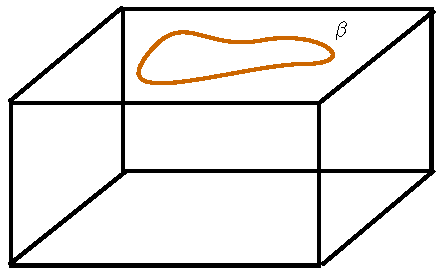
\includegraphics{box_beta_loop.pdf}
\caption{ \label{box_beta_loop} \ethan{I think this figure isn't needed anymore} A sketch of the setup used when considering a shadow world construction which hosts a closed $\beta$ loop on its surface. Restricting the theory to the submanifold defined by this loop produces a result equivalent to the Kitaev wire. \ethan{dave may want to redo}}
\end{figure}
\end{comment}


To summarize, we showed that strands of q-type objects are intimately related to the Kitaev chain. 
One can think of the string net Hamiltonian (defined in Section~\ref{def_sect}) for the $C_2$ theory as describing a phase of fluctuating Kitaev wires, a point of view adopted in \cite{tarantino2016,ware2016,kapustin2017}.
We also noted that fermion condensation is closely tied with the Jordan-Wigner transformation, as one can readily check by looking at looking at the anyon spin chains based on $A_3$ and $A_3/\psi = C_2$.
%\dave{I'm very tempted at making that bit a little more precise since it is very cool, and as far as I know not fully explained anywhere.}.
%\dave{Less tempted today.}
With the one-dimensional Hamiltonian at hand, we showed how to explicitly construct the MPS for the ground state wavefunctions in this graphical language, recovering the same MPS as \cite{fidkowski2011,turzillo2016,bultinck2017b}.
%\ethan{I still don't see how these are the same MPS. %Our matrices are different (we have $A^4$s), and our hilbert space is also different %(their physical index runs over $\unit,\beta$, while we treat the odd and even parts %of $\beta$ separately).}
%\dave{Can you refer to an exact equation? 
%I think I found one of the references was using the same matrices up to a gauge transformation, but I forget which ref and where (you can always send $A_i \tp U_i^{\dagger} A_i U_{i+1}$).
%}
%\ethan{actually, I think this is just me being a bit thick and just not understanding the point of this approach to MPS, but I see it now. I retract my earlier objection} 
We also note that the same MPS can be found by taking a disk with two marked points labeled by a q-type strand and $n-2$ marked points labeled by the identity 
and employing the shadow world construction outlined in Section~\ref{shadowworld}.
%\dave{Anything else we need in the summary paragraph? I'm also happy to remove some of the stuff.}


\begin{comment}
\ethan{commented this out; pretty much all of it appears elsewhere in the section}
\dave{Notation needs to be updated. 
We could also try to condense this a little.}
Finally, we point out that this $(1+1)$-dimensional example sheds some light on the $(2+1)$-dimensional examples 
considered in the majority of the paper. 
For example, in the simple case of the $C_2$ theory, it allows us to make the observation that
$\beta$ strings are equivalent to fluctuating Kitaev chains in their topological phase. 
We can see this by considering a state in the $C_2$ theory constructed 
from the shadow world approach described in the previous section with $v_0 = \emptyset$ and $v_1$\dave{I think the notation is outdated} a state 
with a single closed $\beta$ loop which inherits spin structure $X$, see Figure \ref{box_beta_loop}.
The degrees of freedom in this state are the same as 
the degrees of freedom in the Kitaev chain constructed over $S^1_X$, 
where we identify each vertex Hilbert space with a pair $a_{2j}\tp a_{2j+1}$ of Majoranna\dave{also outdated.}
variables connecting two adjacent physical sites. 
Furthermore, the Hamiltonian defined in Section \ref{Super_pivotal_Hamiltonian} is the same as the Kitaev 
chain Hamiltonian \eqref{staggered_H} when acting on $v_1$. 
The vertex and plaquette terms are trivially satisfied by the choice of $v_1$, and so we only need to focus 
on the edge term $\lambda_e \sum_{e\in \mce} (1-D_e)$. As described in Section \ref{edge_term}, 
the operator $D_e$ changes the fermion parity of the vertices $v,v'$ at the ends of the edge $e$, provided
that $e$ is colored by a $\beta$ line. 
This is exactly the same process implemented by the Kitaev wire Hamiltonian: both Hamiltonians
 are responsible for ``sliding'' fermions along $\beta$ strings.  
\end{comment}


%%% let's just not deal with this
\begin{comment}
To summarize, states in the $C_2$ theory are formed from superpositions of fluctuating Kitaev chains, which in our case are exactly equivalent to $\beta$ strings. 
With these remarks in mind, it 
is natural to view q-type strings in more general $(2+1)$-dimensional super fusion categories 
as different types of fluctuating Kitaev chains, which is a point of view adopted in \cite{tarantino2016,ware2016,kapustin2017}. 
There are several pieces of evidence for this: the fermion parity of a closed q-type string 
depends only on the string's homology class and is determined by the spin structure it inherits, 
and in the simplest case of the $C_2$ theory, q-type strings literally are Kitaev chains, as shown 
above. 

\dave{I think the concensus is to remove this, but we can discuss it if we like.}
However, we have seen examples of theories in which q-type strings do not behave like Kitaev wires.
\dave{I think I'm not so convinced of this anymore. 
It seems like they just don't behave as free-fermion Kitaev wires, or something like that -- which is kind of expected. 
We could think about that more, or modify/remove the sentence/paragraph. 
Ethan, did you have a chance to do the $\halfesix$ calculation we chatted about the other day? 
i.e., check for a zero mode living at the junction of three $\rho$ strands when the Hamiltonian is written in the language of this section?
I'm pretty sure there has to be one, and could explain some of the mystery of $\halfesix$.}
In such theories (like the $SO(3)_6$ and $\halfesix$ examples considered earlier), two q-type
strings can fuse to a q-type string, and two m-type strings can fuse to a q-type. 
If all open q-type strings hosted Majorana zero modes at their ends, such fusion rules would 
be disallowed, since the number of Majorana zero modes must be preserved modulo 2.

\end{comment}

 